```latex
% Options for packages loaded elsewhere
\PassOptionsToPackage{unicode}{hyperref}
\PassOptionsToPackage{hyphens}{url}
\documentclass[
]{article}
\usepackage{xcolor}
\usepackage{amsmath,amssymb}
\setcounter{secnumdepth}{-\maxdimen} % remove section numbering
\usepackage{iftex}
\ifPDFTeX
  \usepackage[T1]{fontenc}
  \usepackage[utf8]{inputenc}
  \usepackage{textcomp} % provide euro and other symbols
else % if luatex or xetex
  \usepackage{unicode-math} % this also loads fontspec
  \defaultfontfeatures{Scale=MatchLowercase}
  \defaultfontfeatures[\rmfamily]{Ligatures=TeX,Scale=1}
\fi
\usepackage{lmodern}
\ifPDFTeX\else
  % xetex/luatex font selection
\fi
% Use upquote if available, for straight quotes in verbatim environments
\IfFileExists{upquote.sty}{\usepackage{upquote}}{}
\IfFileExists{microtype.sty}{% use microtype if available
  \usepackage[]{microtype}
  \UseMicrotypeSet[protrusion]{basicmath} % disable protrusion for tt fonts
}{}
\makeatletter
\@ifundefined{KOMAClassName}{% if non-KOMA class
  \IfFileExists{parskip.sty}{%
    \usepackage{parskip}
  }{% else
    \setlength{\parindent}{0pt}
    \setlength{\parskip}{6pt plus 2pt minus 1pt}}
}{% if KOMA class
  \KOMAoptions{parskip=half}}
\makeatother
\usepackage{graphicx}
\makeatletter
\newsavebox\pandoc@box
\newcommand*\pandocbounded[1]{% scales image to fit in text height/width
  \sbox\pandoc@box{#1}%
  \Gscale@div\@tempa{\textheight}{\dimexpr\ht\pandoc@box+\dp\pandoc@box\relax}%
  \Gscale@div\@tempb{\linewidth}{\wd\pandoc@box}%
  \ifdim\@tempb\p@<\@tempa\p@\let\@tempa\@tempb\fi% select the smaller of both
  \ifdim\@tempa\p@<\p@\scalebox{\@tempa}{\usebox\pandoc@box}%
  \else\usebox{\pandoc@box}%
  \fi%
}
% Set default figure placement to htbp
\def\fps@figure{htbp}
\makeatother
\setlength{\emergencystretch}{3em} % prevent overfull lines
\providecommand{\tightlist}{%
  \setlength{\itemsep}{0pt}\setlength{\parskip}{0pt}}
\usepackage{bookmark}
\IfFileExists{xurl.sty}{\usepackage{xurl}}{} % add URL line breaks if available
\urlstyle{same}
\hypersetup{
  hidelinks,
  pdfcreator={LaTeX via pandoc}}

\title{Pythagorean Theorem Proof}
\author{}
\date{}

\begin{document}

\maketitle

\begin{abstract}
This paper presents a concise, geometry-based framework for proving the Pythagorean theorem, establishing that in a right triangle with legs $a$ and $b$ and hypotenuse $c$, the relation $a^2 + b^2 = c^2$ holds. The approach emphasizes constructions with squares on the sides and congruent triangles to compare areas, providing a purely geometric argument that relates the areas of figures built from the legs to the square on the hypotenuse. The abstract outlines the problem, the central hypothesis, and the planned logical sequence—definitions, lemmas, and a diagrammatic reasoning path—that will underpin a rigorous proof. The presentation is tailored for a conference audience, focusing on clarity of the square-area decomposition and triangle congruences, while avoiding numerical computation or empirical results at this stage. The abstract serves as a roadmap for the Introduction, the forthcoming proof skeleton, and the discussion of necessary geometric principles.
\end{abstract}

\section{Introduction}
In a right triangle, the hypotenuse is the side opposite the right angle, and its length is determined by the lengths of the two legs. If the legs have lengths $a$ and $b$ and the hypotenuse has length $c$, the Pythagorean relation states that $a^2 + b^2 = c^2$, a foundational identity in Euclidean geometry. The present work aims to establish this relation through a constructive geometric proof that uses squares erected on the sides and assemblies of triangles, aligning with the hypothesis that the theorem can be derived from square-and-triangle constructions. The following diagram illustrates the configuration used in the argument:

\begin{figure}[htbp]
  \centering
  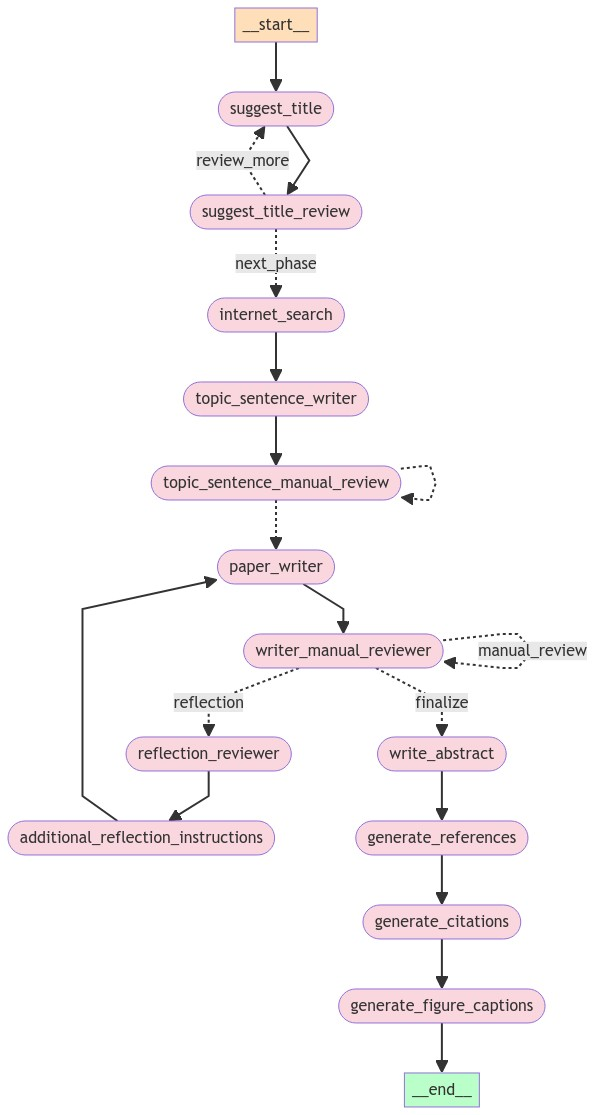
\includegraphics[width=\linewidth, keepaspectratio]{multi-agent.jpeg}
  \caption{Figure 1: multi-agent.jpeg}
  \label{fig:multi-agent}
\end{figure}

\section{Results}
No paper results are given.

\section{References}
No references are provided.

\end{document}
```